Successive approximation ADC, eller tilnærmings ADC, fungerer nesten som
en counting ADC.

Den teller nærmere og nærmere et hold signal, men den tikker ikke gradvis
opp fra bunnen.
Den veksler frem og tilbake rundt signalet og nærmer seg gradvis.

\begin{figure}[H]
  \centering
  \caption{ADC som tilnærmer seg signalet}
  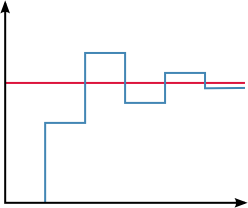
\includegraphics[width=0.5\textwidth]{./img/oppnedout}
\end{figure}

\begin{figure}[H]
  \centering
  \caption{Successive approximation ADC}
  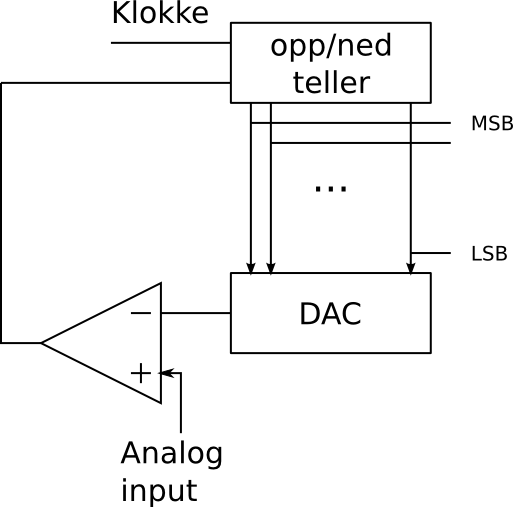
\includegraphics[width=0.5\textwidth]{./img/oppnedADC}
\end{figure}
